\documentclass[11pt]{article}
\renewcommand{\familydefault}{\sfdefault}
\newcommand{\photfluxucd}{phot.flux.density}

\newcommand{\httitle}[1]{}
\newcommand{\htwidth}[1]{}
\newcommand{\hdebug}{}
\newcommand{\htzero}{}
\newcommand{\htmtitle}[2]{\parbox{6.0in}{ \bf \huge #1 \\  \Large  #2}}
\newcommand{\htpart}[1]{\centerline{\bf #1}}
\newcommand{\heol}{} % HTML ignore rest of line

%  Stub
%\newcommand{\htmladdnormallink}[1]{}


\usepackage[usenames]{color}
\usepackage{graphicx}
\usepackage{psfig}
\usepackage{epsf}
\usepackage{html}
\usepackage{lscape}

\textheight 9.0in
\textwidth 6.0in
\hoffset -0.7in
\voffset -0.5in

\newcommand{\lcaret}{\mbox{$<$}}
\newcommand{\rcaret}{\mbox{$>$}}
\newcommand{\link}[1]{{\color{dblue}\htmladdnormallink{#1}{}\par}}
\newcommand{\m}[1]{\mbox{#1}}
\newcommand{\change}[1]{{ #1}}
\newsavebox{\fmbox}
\newenvironment{fmpage}
     {\begin{lrbox}{\fmbox}\begin{minipage}{6.5in}}
     {\end{minipage}\end{lrbox}\colorbox{iblue}{\fbox{\usebox{\fmbox}}}}

\newenvironment{fmlpage}
     {\begin{lrbox}{\fmbox}\begin{minipage}{9.3in}}
     {\end{minipage}\end{lrbox}\colorbox{iblue}{\fbox{\usebox{\fmbox}}}}

\newenvironment{fmppage}
     {\begin{lrbox}{\fmbox}\begin{minipage}{6.5in}}
     {\end{minipage}\end{lrbox}\colorbox{ipink}{\fbox{\usebox{\fmbox}}}}

\httitle{IVOA Photometry Data Model}{}

\begin{document}

\vskip -1in
\heol
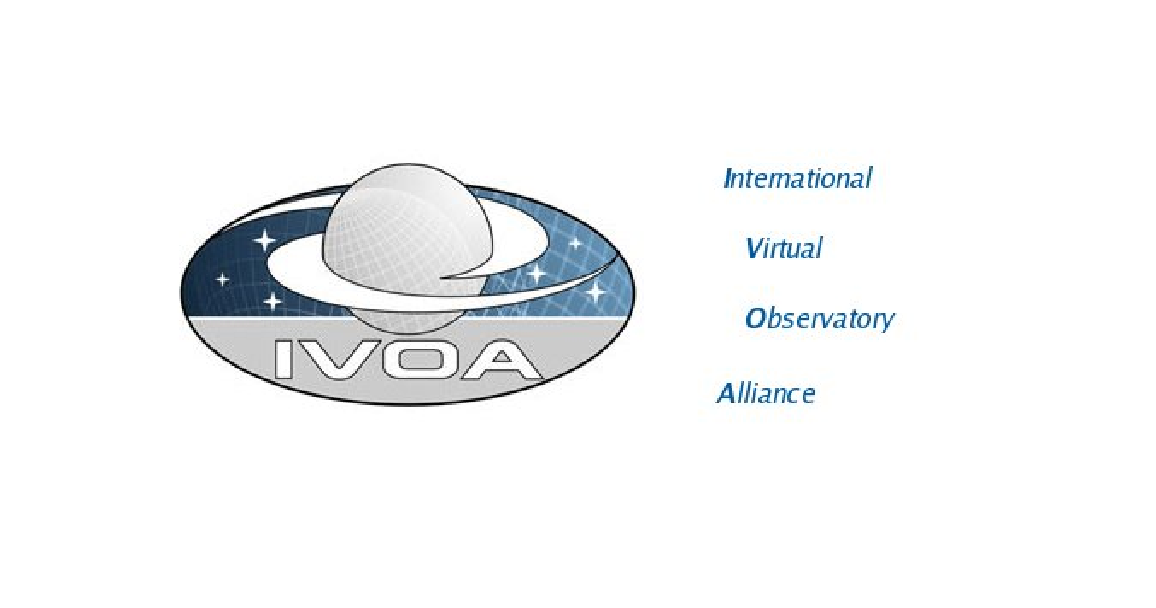
\psfig{file=ivoa.ps,width=5.0in}

\definecolor{ipink}{rgb}{1.0,0.937,0.957}
\definecolor{dblue}{rgb}{0.60,0.60,1.0}
\definecolor{ddblue}{rgb}{0.20,0.20,1.0}
\definecolor{iblue}{rgb}{0.9,0.9,1.0}
\color{dblue}
\vskip 0.2in
\par\noindent \htmtitle{IVOA Photometry Data Model}{Version 0.2}
\Large
\vskip 0.1in
\par\noindent{\bf IVOA Note}
\color{Black}
\vskip 0.2in

\normalsize

\par\noindent{\bf V0.2 Mod 0}

{ 
\color{dblue}
\htmladdnormallink{http://www.ivoa.net/Documents/TBD}{}


\par\noindent{\bf Latest version:}
}

{\color{dblue}
\link{http://www.ivoa.net/Documents/latest/SED.html}
}

%\par\noindent{\bf Previous versions:}

%{\color{dblue}
%\link{http://www.ivoa.net/Documents/REC/DM/SpectrumDM-20090515.pdf}
%}

\vskip 0.2in

\noindent{\bf Editors:}

Jonathan McDowell, Pedro Osuna

\noindent{\bf Contributors:}

Jonathan McDowell, Doug Tody, Pedro Osuna, Joe Mazzarella, Raffaele D'Abrusco, ...?
and the IVOA Data Access Layer and Data Model Working Groups.


\begin{abstract}

We present a data model for photometry, intended for use in
conjunction with the IVOA Spectral Energy Distributions (SED) 
and Spectrum data models.

\end{abstract}

\clearpage

\subsection*{ Status of this document }

This is a draft for discussion among the relevant VAO and IVOA working groups.

This document has been developed with support from the National Science 
Foundation and NASA.

The {\bf Virtual Observatory (VO)} is general term for a collection of
federated resources that can be used to conduct astronomical research,
education, and outreach. 

The {\bf International Virtual Observatory Alliance
(IVOA)} (\link{http://www.ivoa.net}) is a global collaboration of separately
funded projects to develop standards and infrastructure that enable VO
applications.

\clearpage

\tableofcontents

\newpage

\addcontentsline{toc}{part}{Part 1 - Photometry Data Model}

\htzero

{\Large
\vfill
\htpart{Part 1: Photometry Data Model}
\vfill
}
\newpage
\section{Introduction and Motivation}

The IVOA has identified creation and analysis of spectral energy distributions
as a key science capability desired in the VO.
In this document we present a proposed abstraction for
photometry data to be used in 
spectral energy distributions.

\subsection{Change Log}

\begin{verbatim}
2010 Nov 4  Initial draft.
\end{verbatim}

\clearpage

\section{Photometric data}

\psfig{file=photdm.ps,width=6.0in}


\end{document}

